% Verified numerical results and the conditional first-stage decision.
630 行方法结果、126 条完整历史均通过独立重算，全部位置／速度输出有限；
CSV 与重算的最大绝对差为 $3.64\times10^{-12}$。
\textbf{有限数值不等于可靠定位}：InEKF 与 ESKF 的最坏位置误差分别约 22.0 km、8.07 km，
均保留为失败，不裁去后半轨迹。

\begin{center}
\begin{tabular}{lrrr}
\toprule
方法&LOSO 成功／24&留出成功／90&中断成功／12\\\midrule
InEKF-15&17&62&5\\
ESKF-15&20&76&3\\
捕获初始化&20&75&8\\
捕获初始化＋中断重置&20&75&10\\
完整 deep&19&61&2\\\bottomrule
\end{tabular}
\end{center}

留出组完整位置 RMSE 中位数：捕获初始化 0.331 m、deep 0.375 m；
末 5 秒分别 0.151 m、0.179 m。
按日志等权的配对完整 RMSE 相对变化为 deep 高 10.76\%，
日志重采样 95\% 区间为 $[1.64,17.02]\%$。
成功率差为 $-15.56$ 个百分点，但六日志重采样区间 $[-61.11,28.89]$ 跨零；
不将相关的 90 个用例当独立证据。
双方均成功的 48 对中，日志等权恢复时间差为 deep 慢 3.75 s，
可用五日志的区间为 $[0.006,11.20]$ s；条件化统计不能代表全部失败用例。

deep \textbf{存在局部收益}：留出 square 日志成功 13/15，而捕获初始化为 0/15；
同时 octagon／star 分别由简化方案的 15/15 降为 deep 的 2/15、1/15。
与简化初始化配对，deep 独有成功 13 对、简化独有成功 27 对。
90／180 度扰动下 ESKF 均 6/6，简化初始化均 5/6，deep 为 4/6、5/6；
普通 InEKF 为 4/6、3/6。这是当前零杆臂 TWR 共同模型结果，不能推广为对原文 TDoA 的否定。

中断后 deep／简化重置的末 5 秒位置 RMSE 中位数为 9.235／0.151 m。
deep 两次成功均来自 square，恰为重置失败的两例；重置其余十例成功，deep 全部失败。
双方没有共同成功对，因此\textbf{不存在可计算的配对成功恢复时间差}。
分别报告的成功用例中位恢复时间为 11.79／11.10 s，不能据此称速度相当。

\textbf{第一阶段工程与比较工作完成，第二阶段的进入条件未满足。}
保留完整 deep 及其局部收益证据，但暂停以当前双滤波器为核心的稳定优势叙事。
目前优先基线是固定捕获初始化、测距恢复后再次捕获与单不变 tracker。
它仍有 square 失败和正常初期峰值，尚未达到普遍可靠定位。
若继续研究，应先解释“square 改善、octagon／star 退化、长中断捕获漂移”这一具体机制，
再以独立日期与锚点几何检验；本轮没有新增收敛定理、NEES 或目标硬件实时证据。

\clearpage
\section{可观察结果}
\begin{center}
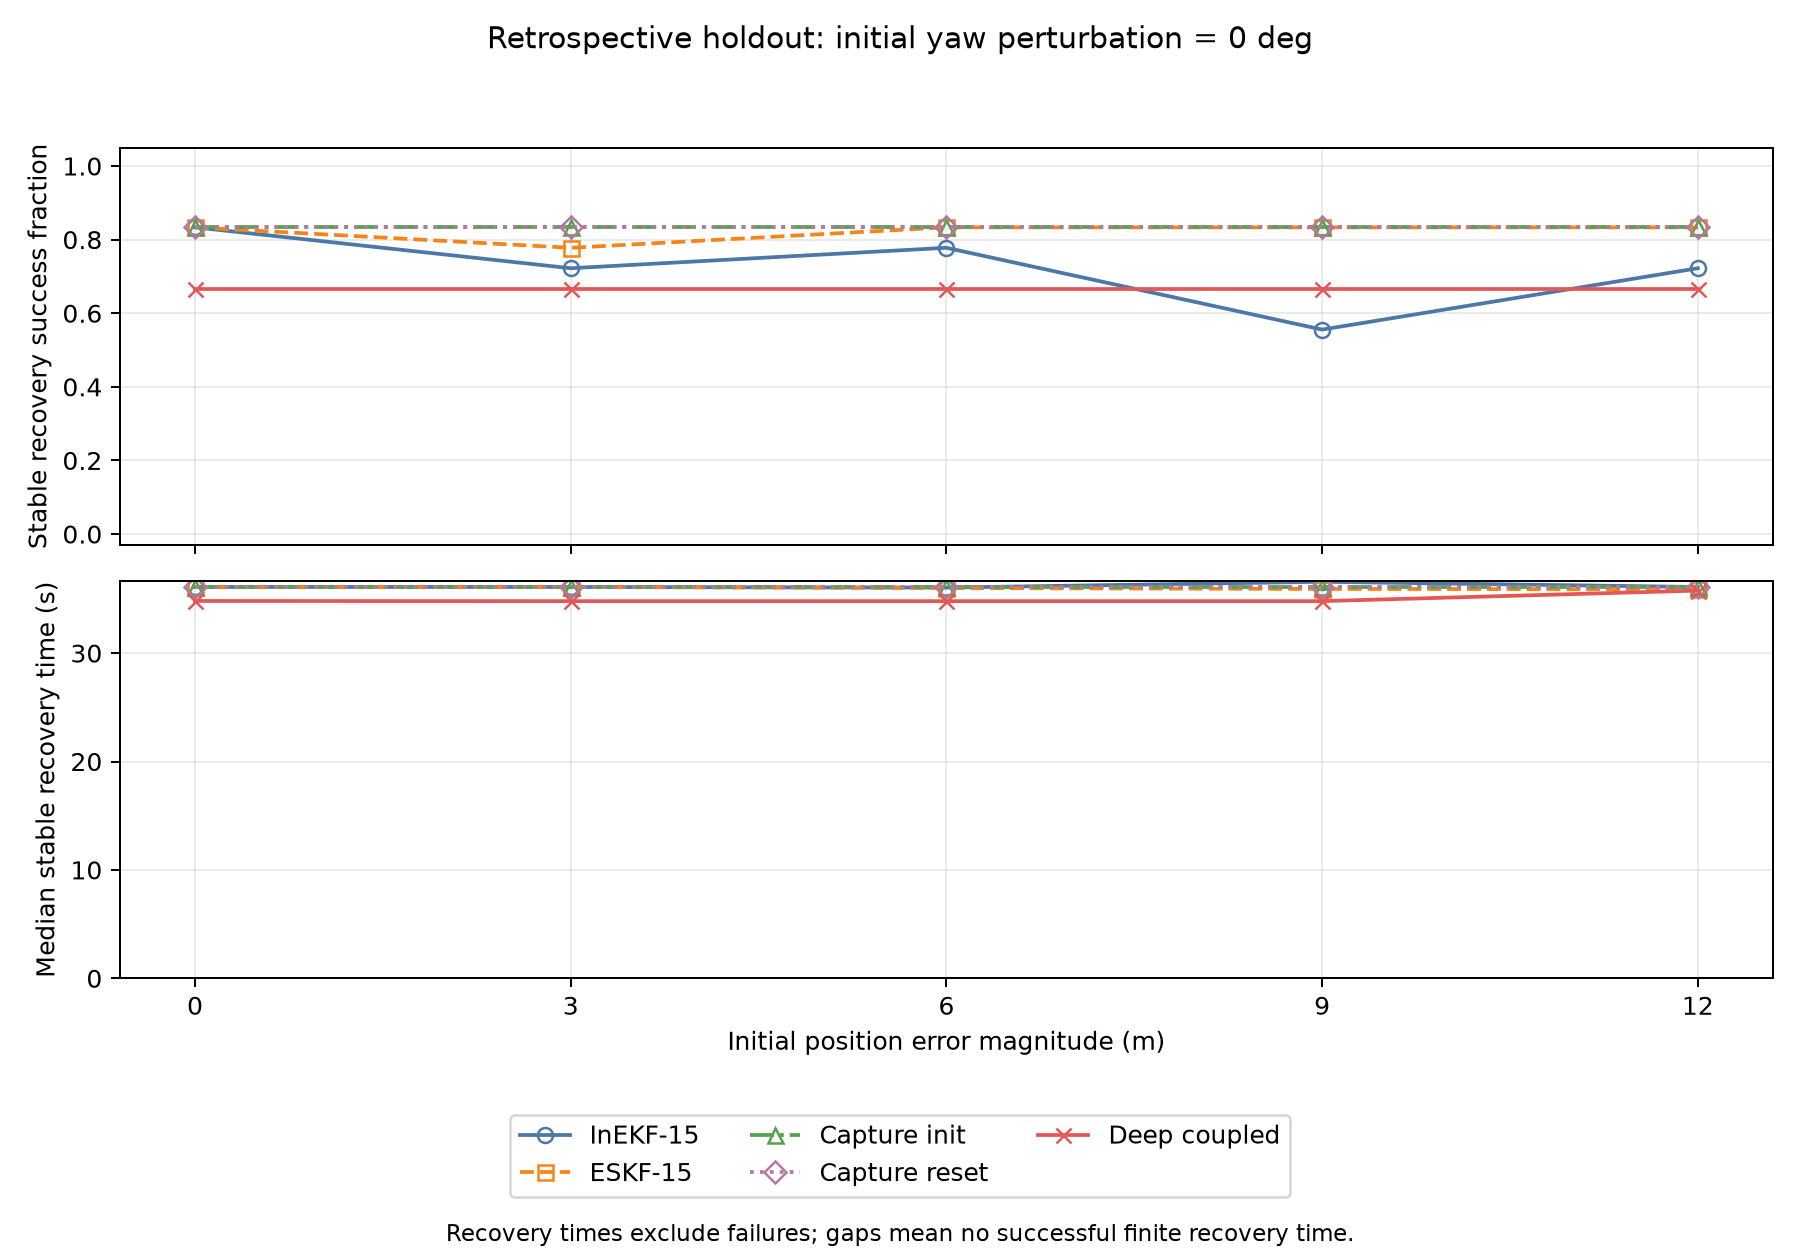
\includegraphics[width=0.87\linewidth]{../imu-uwb-inekf/results/roadmap_stage1_20261104_final/holdout_capture_domain.png}
\end{center}
固定标定留出组的初差域。0 m 为六条件，非零幅度均为六日志乘三方向。
下图仅对成功用例统计，约 35--36 秒的终段稳定时间不等于首次达到阈值。

\begin{center}
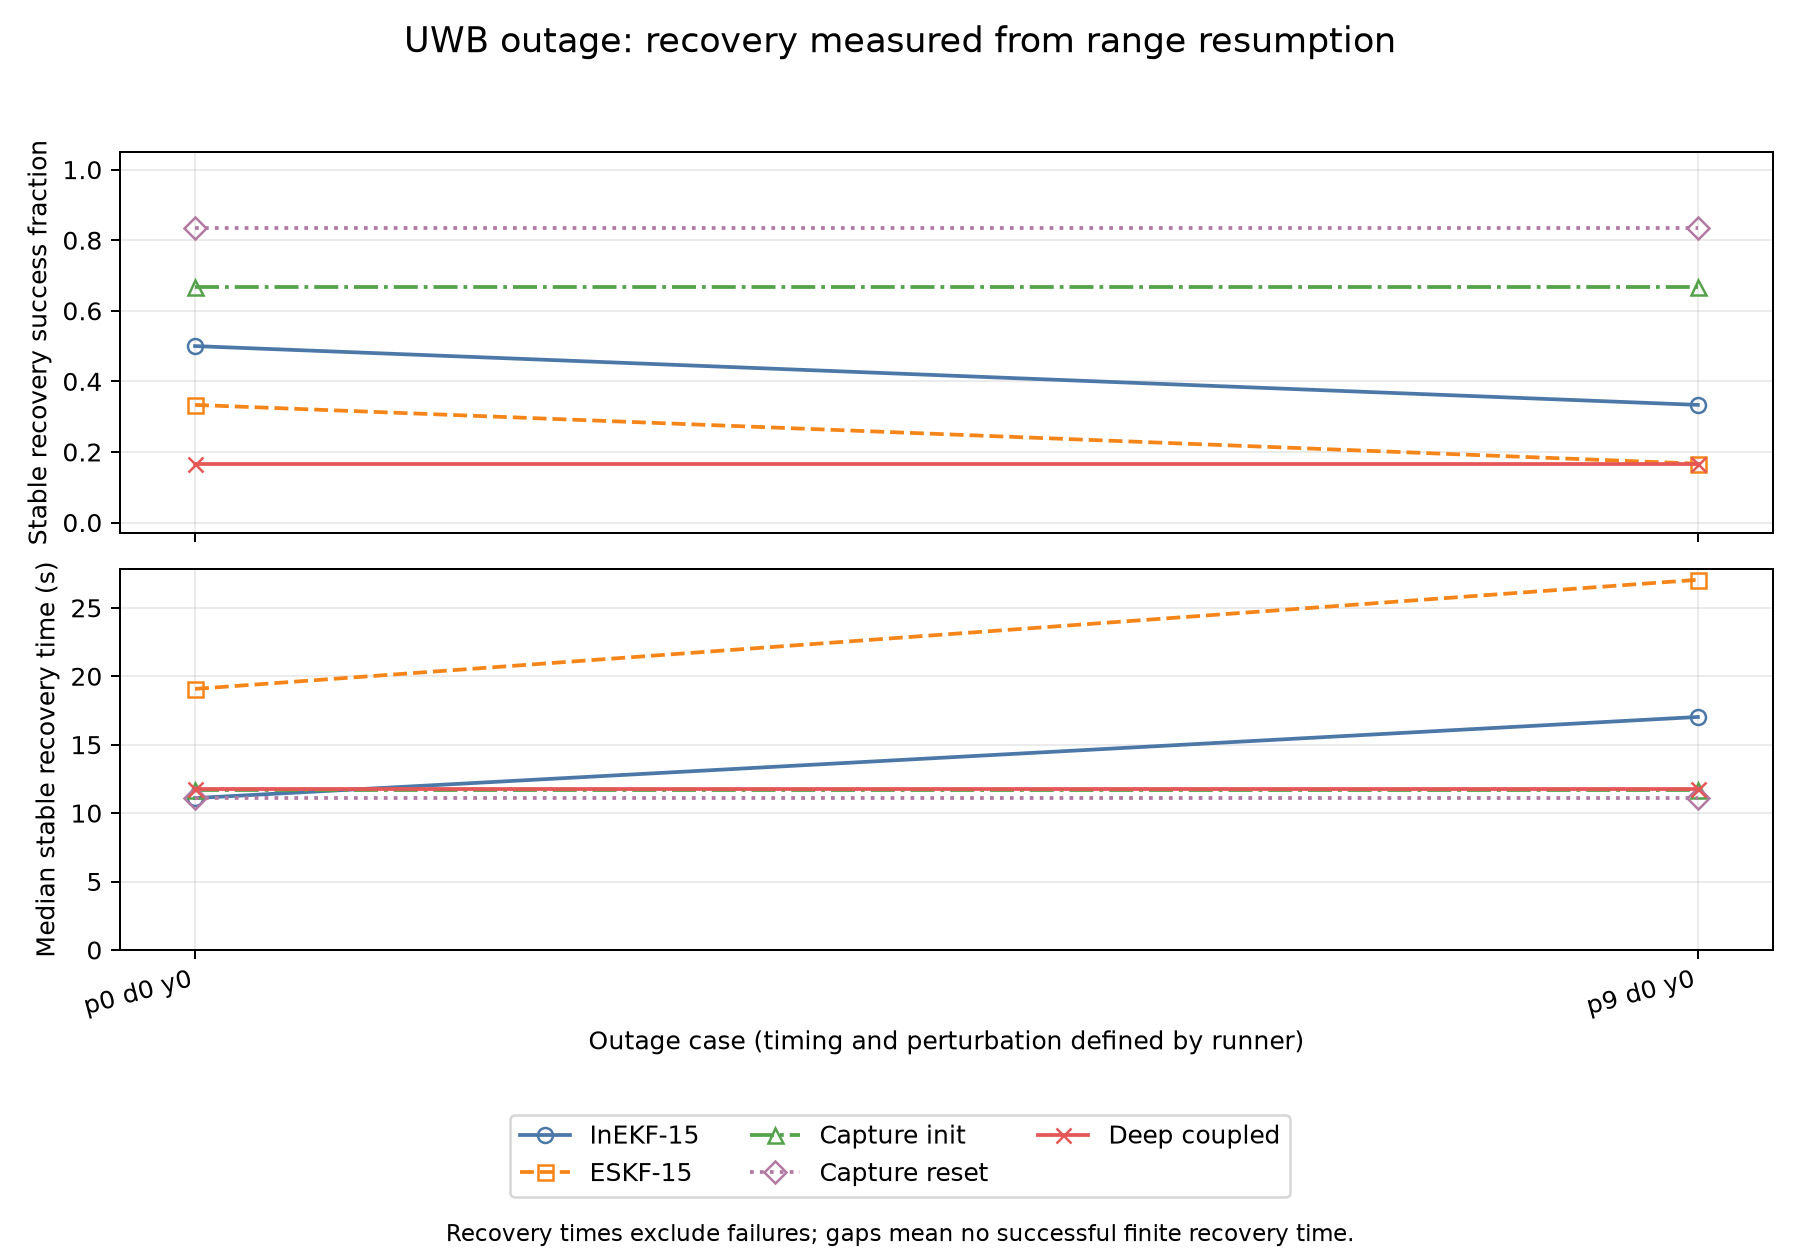
\includegraphics[width=0.87\linewidth]{../imu-uwb-inekf/results/roadmap_stage1_20261104_final/outage_recovery.png}
\end{center}
测距中断 15--25 秒；恢复时间从 25 秒起算，每组六条件。
失败不会获赋一个虚构恢复时间。

\clearpage
\section{失败与局部收益并列检查}
\begin{center}
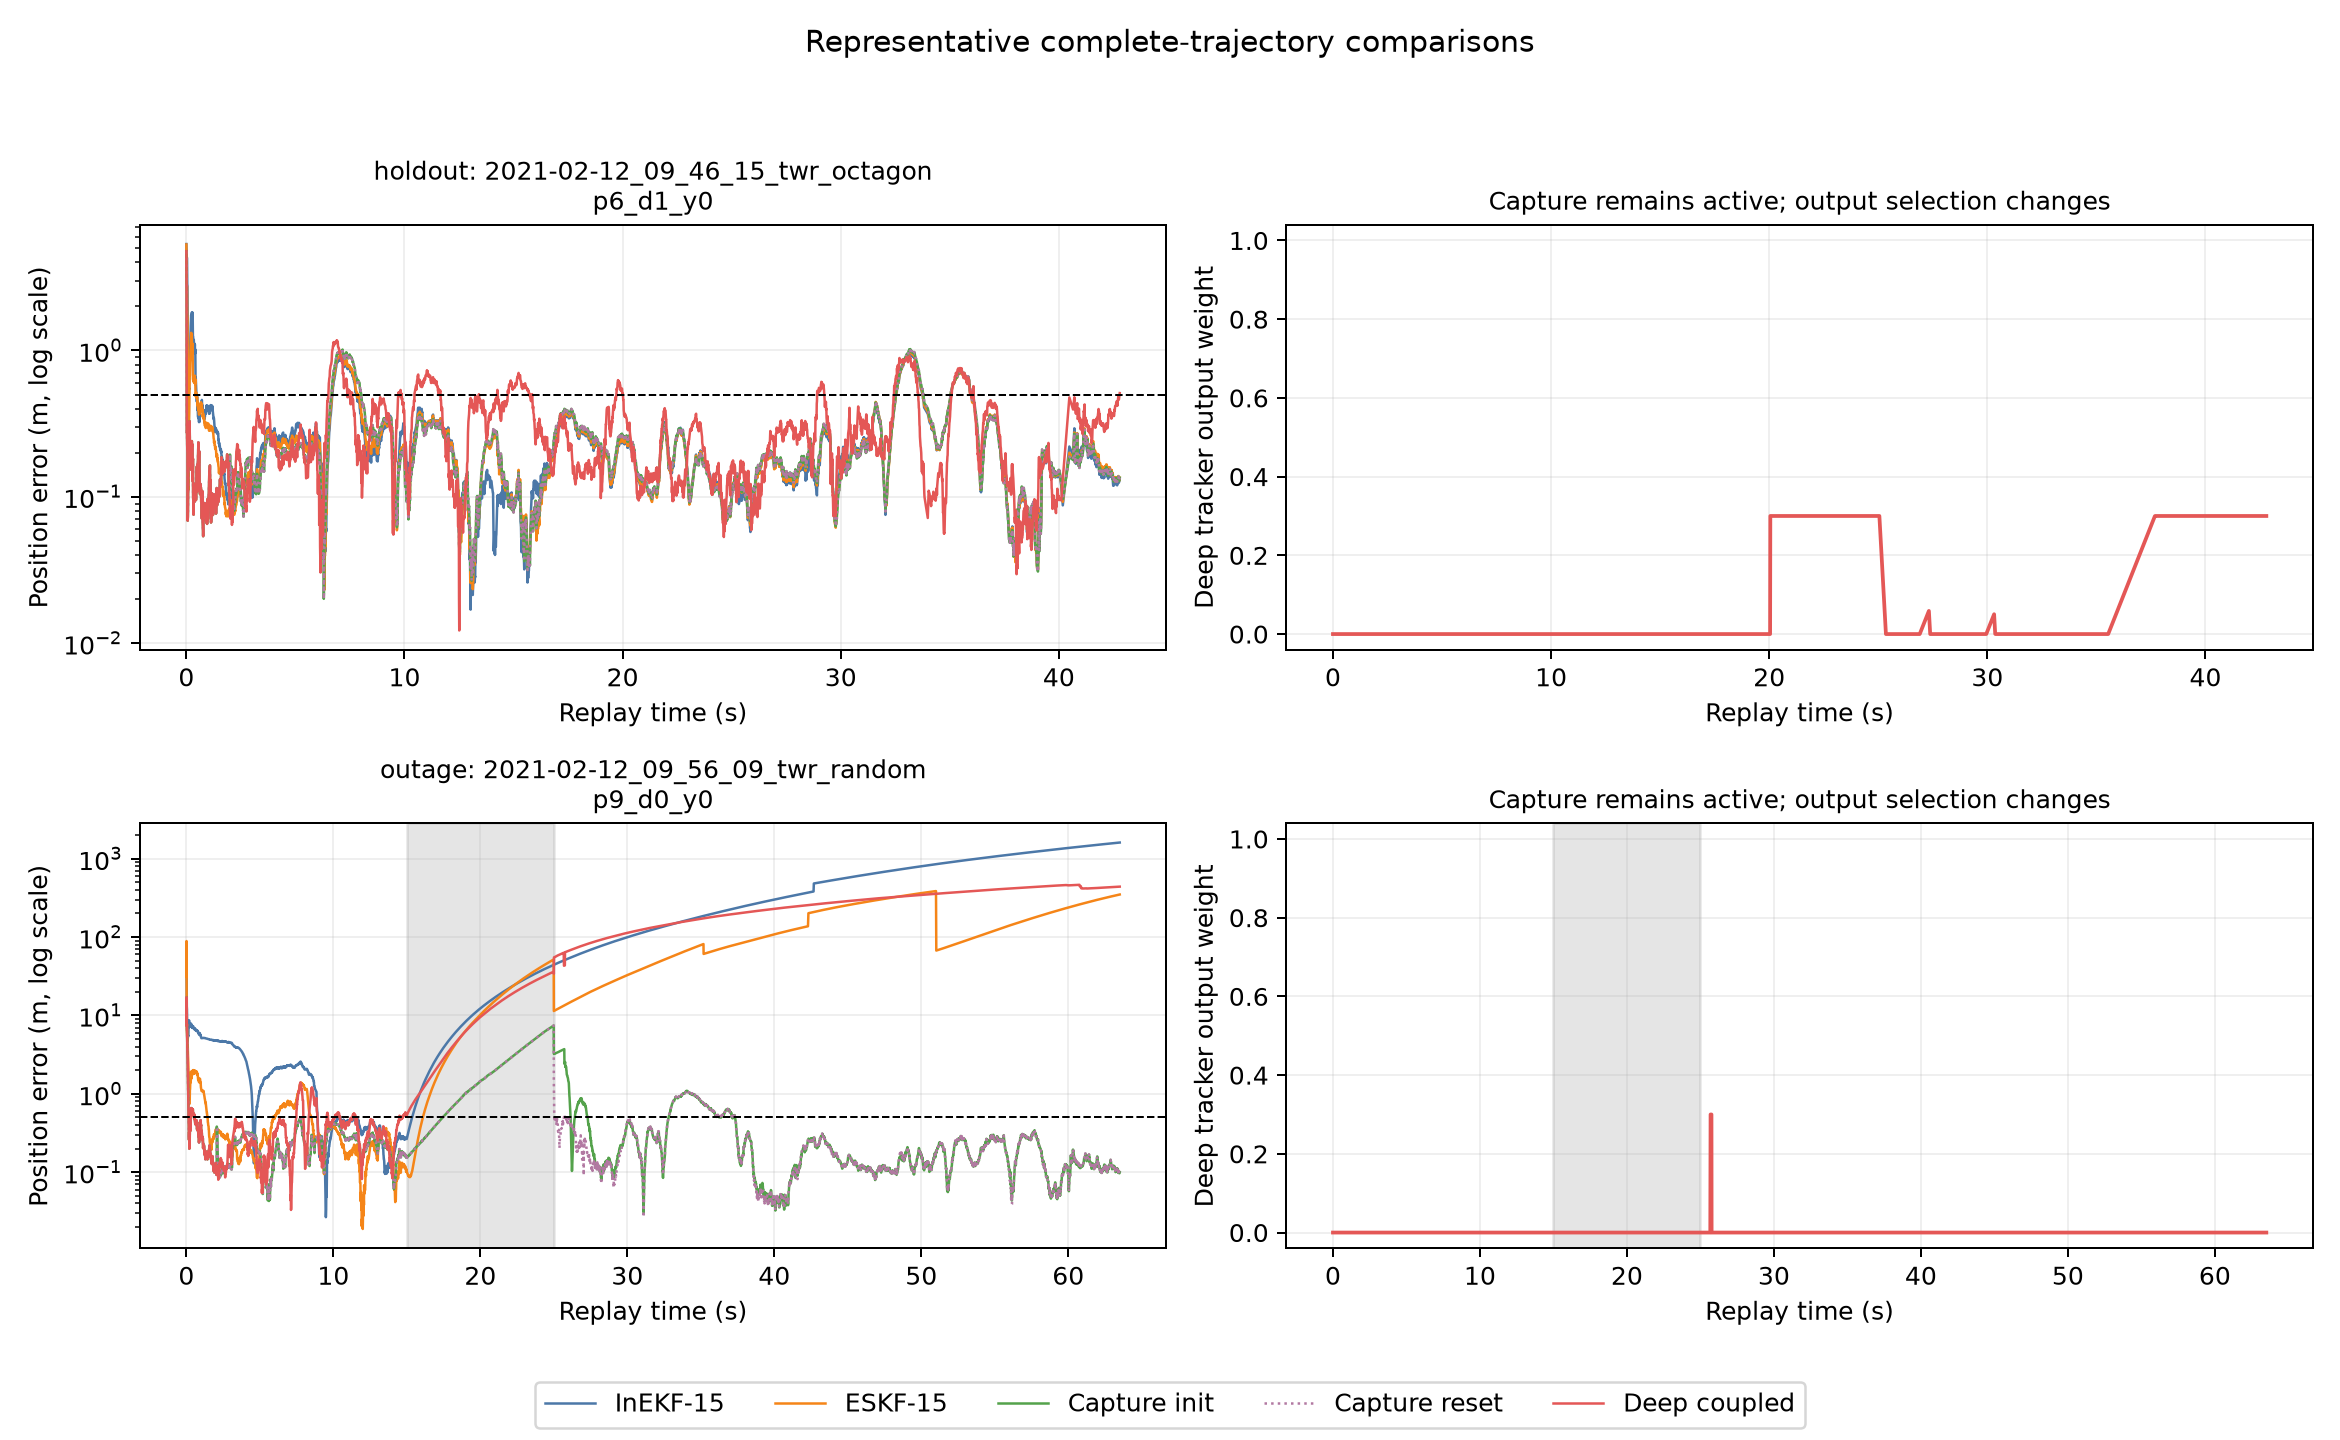
\includegraphics[width=\linewidth]{../imu-uwb-inekf/results/roadmap_stage1_20261104_final/representative_failures.png}
\end{center}
保留完整误差及 deep 输出权重。octagon 的输出混合产生额外末段代价；
random 中断后 deep 权重大多为零，持续捕获仍可漂移。
后者是观察到的现象，不能仅凭曲线证明全部内部因果。

\begin{center}
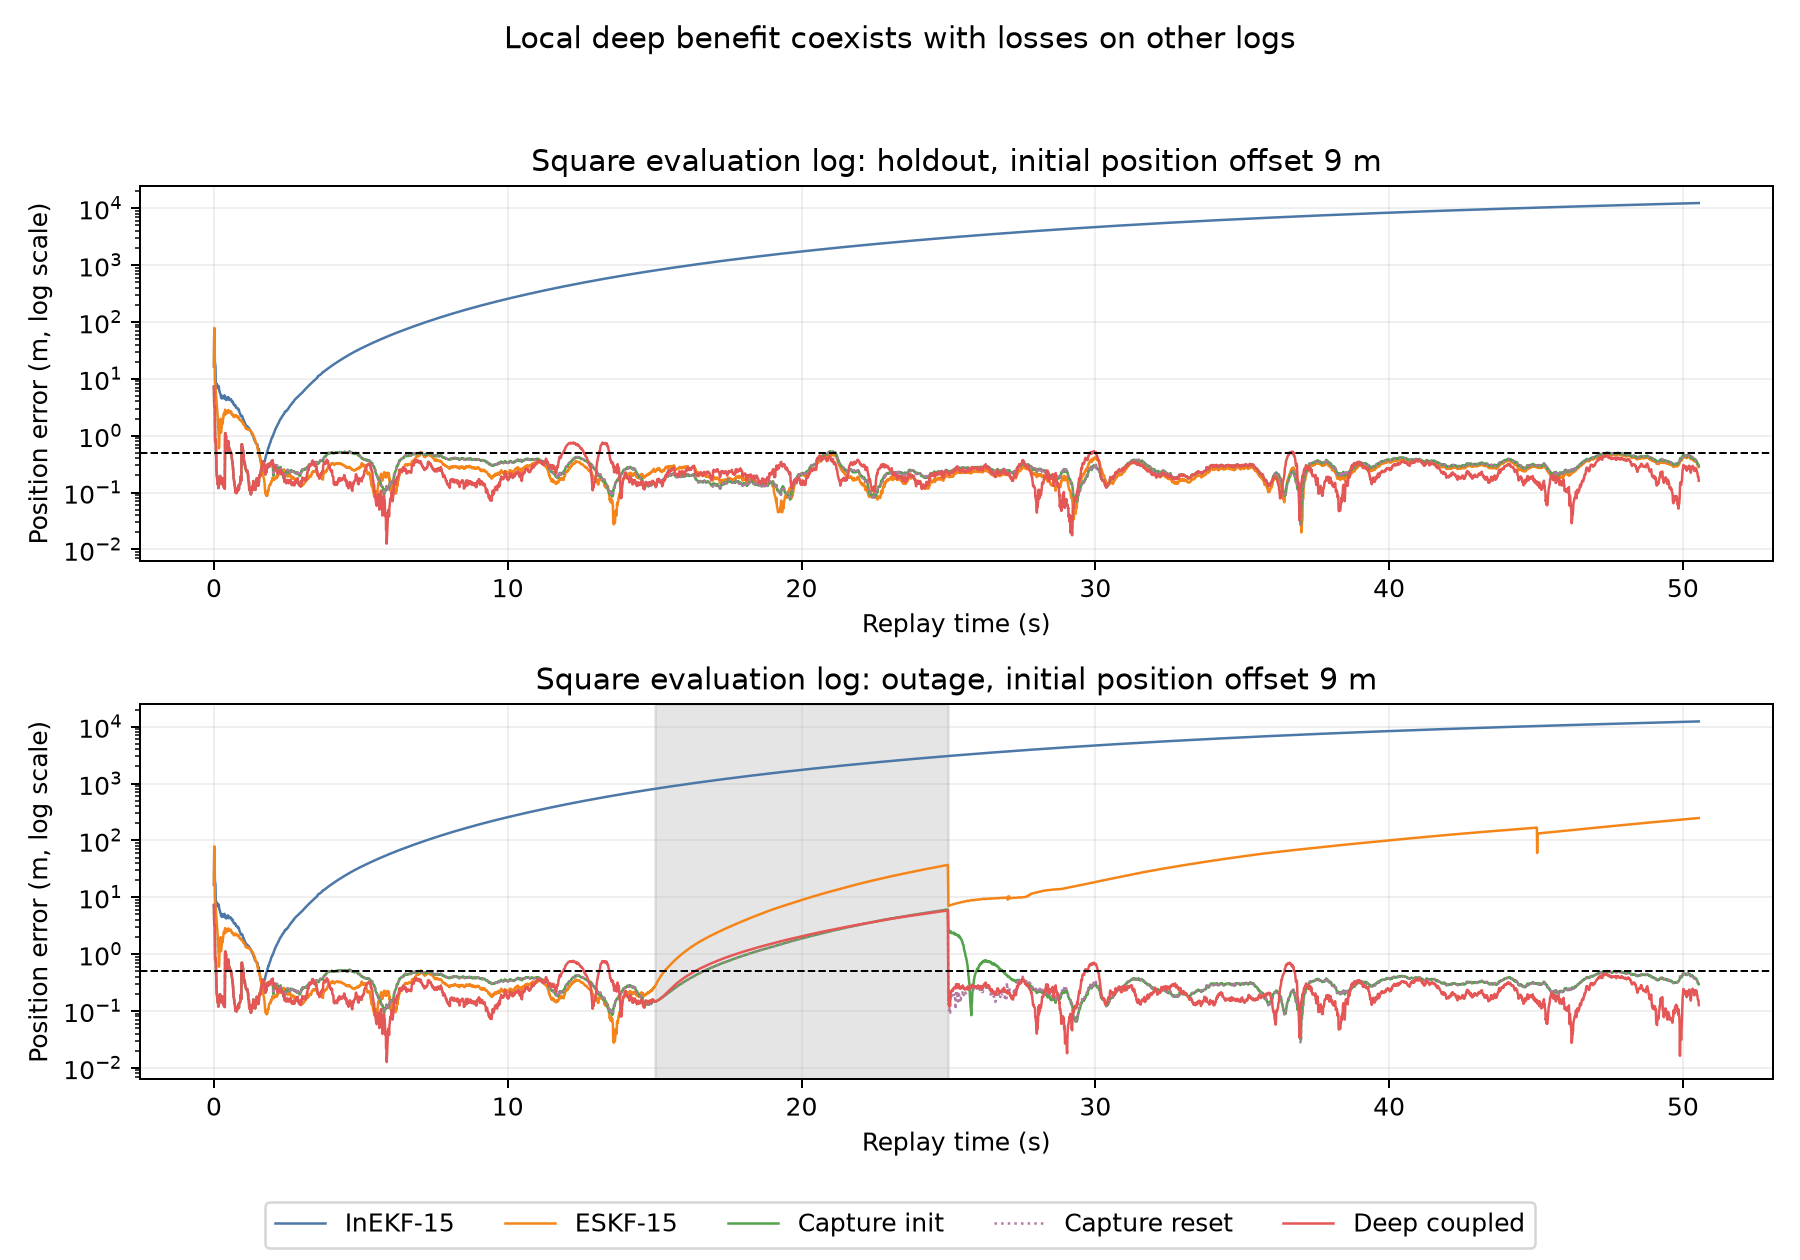
\includegraphics[width=0.83\linewidth]{../imu-uwb-inekf/results/roadmap_stage1_20261104_final/deep_local_gain.png}
\end{center}
square 的 deep 局部收益明确保留；少数阈值峰值可导致简化方案稳定后缀判定失败，
必须结合末段误差、完整峰值和成功率解释。
